%\documentclass[11pt,letterpaper]{article}
\documentclass[[a4paper,landscape]{article}\usepackage[]{graphicx}\usepackage[]{color}
% maxwidth is the original width if it is less than linewidth
% otherwise use linewidth (to make sure the graphics do not exceed the margin)
\makeatletter
\def\maxwidth{ %
  \ifdim\Gin@nat@width>\linewidth
    \linewidth
  \else
    \Gin@nat@width
  \fi
}
\makeatother

\definecolor{fgcolor}{rgb}{0.345, 0.345, 0.345}
\newcommand{\hlnum}[1]{\textcolor[rgb]{0.686,0.059,0.569}{#1}}%
\newcommand{\hlstr}[1]{\textcolor[rgb]{0.192,0.494,0.8}{#1}}%
\newcommand{\hlcom}[1]{\textcolor[rgb]{0.678,0.584,0.686}{\textit{#1}}}%
\newcommand{\hlopt}[1]{\textcolor[rgb]{0,0,0}{#1}}%
\newcommand{\hlstd}[1]{\textcolor[rgb]{0.345,0.345,0.345}{#1}}%
\newcommand{\hlkwa}[1]{\textcolor[rgb]{0.161,0.373,0.58}{\textbf{#1}}}%
\newcommand{\hlkwb}[1]{\textcolor[rgb]{0.69,0.353,0.396}{#1}}%
\newcommand{\hlkwc}[1]{\textcolor[rgb]{0.333,0.667,0.333}{#1}}%
\newcommand{\hlkwd}[1]{\textcolor[rgb]{0.737,0.353,0.396}{\textbf{#1}}}%
\let\hlipl\hlkwb

\usepackage{framed}
\makeatletter
\newenvironment{kframe}{%
 \def\at@end@of@kframe{}%
 \ifinner\ifhmode%
  \def\at@end@of@kframe{\end{minipage}}%
  \begin{minipage}{\columnwidth}%
 \fi\fi%
 \def\FrameCommand##1{\hskip\@totalleftmargin \hskip-\fboxsep
 \colorbox{shadecolor}{##1}\hskip-\fboxsep
     % There is no \\@totalrightmargin, so:
     \hskip-\linewidth \hskip-\@totalleftmargin \hskip\columnwidth}%
 \MakeFramed {\advance\hsize-\width
   \@totalleftmargin\z@ \linewidth\hsize
   \@setminipage}}%
 {\par\unskip\endMakeFramed%
 \at@end@of@kframe}
\makeatother

\definecolor{shadecolor}{rgb}{.97, .97, .97}
\definecolor{messagecolor}{rgb}{0, 0, 0}
\definecolor{warningcolor}{rgb}{1, 0, 1}
\definecolor{errorcolor}{rgb}{1, 0, 0}
\newenvironment{knitrout}{}{} % an empty environment to be redefined in TeX

\usepackage{alltt}
\usepackage{graphicx}
\usepackage{fancybox}
\usepackage{fancyhdr} %pie de pagina y cabecera
\usepackage[utf8]{inputenc} %solucion del problema de los acentos.
\usepackage{multicol,pst-plot}
\usepackage[left=2cm,right=2cm,top=2cm,bottom=2cm]{geometry}
\usepackage{xcolor}
\usepackage[many]{tcolorbox}
\usepackage{svg}

%%%%%%%%%  ESTILO DOC %%%%%%%%%%%%%%%%%%%%%%%%%%%%%%%%%%%%
\definecolor{meteoblue}{RGB}{0,160,250}



\tcbset{mystyle/.style={
  breakable,
  enhanced,
  outer arc=0pt,
  arc=0pt,
  colframe=meteoblue,
  colback=meteoblue!20,
  attach boxed title to top left,
  boxed title style={
    colback=meteoblue,
    outer arc=0pt,
    arc=0pt,
    },
  title=Example~\thetcbcounter,
  fonttitle=\sffamily
  }
}

\newtcolorbox[auto counter,number within=section]{example}[1][]{
  mystyle,
  title=AVISO,
  }
%%%%%%%%%%%%%%%%%%%%%%%%%%%%%%%%%%%%%%%%%%%%%%%%%%
\pagestyle{fancy}

\fancyhead{}
\fancyhead[L]{\tiny\bfseries The product}
\fancyhead[R]{Alpred}
\fancyhead[C]{\today}
\fancyfoot{}
\fancyfoot[LE,RO]{\thepage}
\fancyfoot[LO,RE]{User Guide}
\fancyfoot[C]{Other information}
\IfFileExists{upquote.sty}{\usepackage{upquote}}{}
\begin{document}

%%%%%%%%%%%CABECERA %%%%%%%%%%%%%%%%%%%%%%%%%%%%%%%
%\pagestyle{plain}
%\begin{flushright}
%Almendricos, Espa\~na\\
%\underline{Alpred, S.L}
%\end{flushright}

%\begin{flushleft}\vspace{-8mm}
%\begin{figure}[h]
%
\includegraphics[width=0.2\textwidth]{/home/raquel/repos/pruebas/informes/meteoredlogo.pdf}
%\end{figure}
%\end{flushleft}

%\vspace{-1mm}
%\textcolor{meteoblue}{\rule{\linewidth}{1mm}}
%%%%%%%%%%%%%%%%%%%%%%%%%%%%%%%%%%%%%%%%%%%%%%%%%%








\begin{center}\vspace{-1cm}
\textcolor{meteoblue}{\textbf{ \huge Prediccion para \textcolor{meteoblue}{Madrid [40.4200;356.3200]} }}\\
\date{\today}
\end{center}

\textcolor{meteoblue}{\rule{\linewidth}{1mm}}

\vspace{2cm}

\vspace{2cm}
\begin{example}
La temperaturea maxima es 12.63 \\
La temperaturea media es 3.5905417
\end{example}

\vspace{2cm}
\begin{example}

La temperaturea maxima es 12.63 \\
La temperaturea media es 3.5905417
\end{example}

\pagestyle{plain}
\begin{figure}
\begin{knitrout}
\definecolor{shadecolor}{rgb}{0.969, 0.969, 0.969}\color{fgcolor}
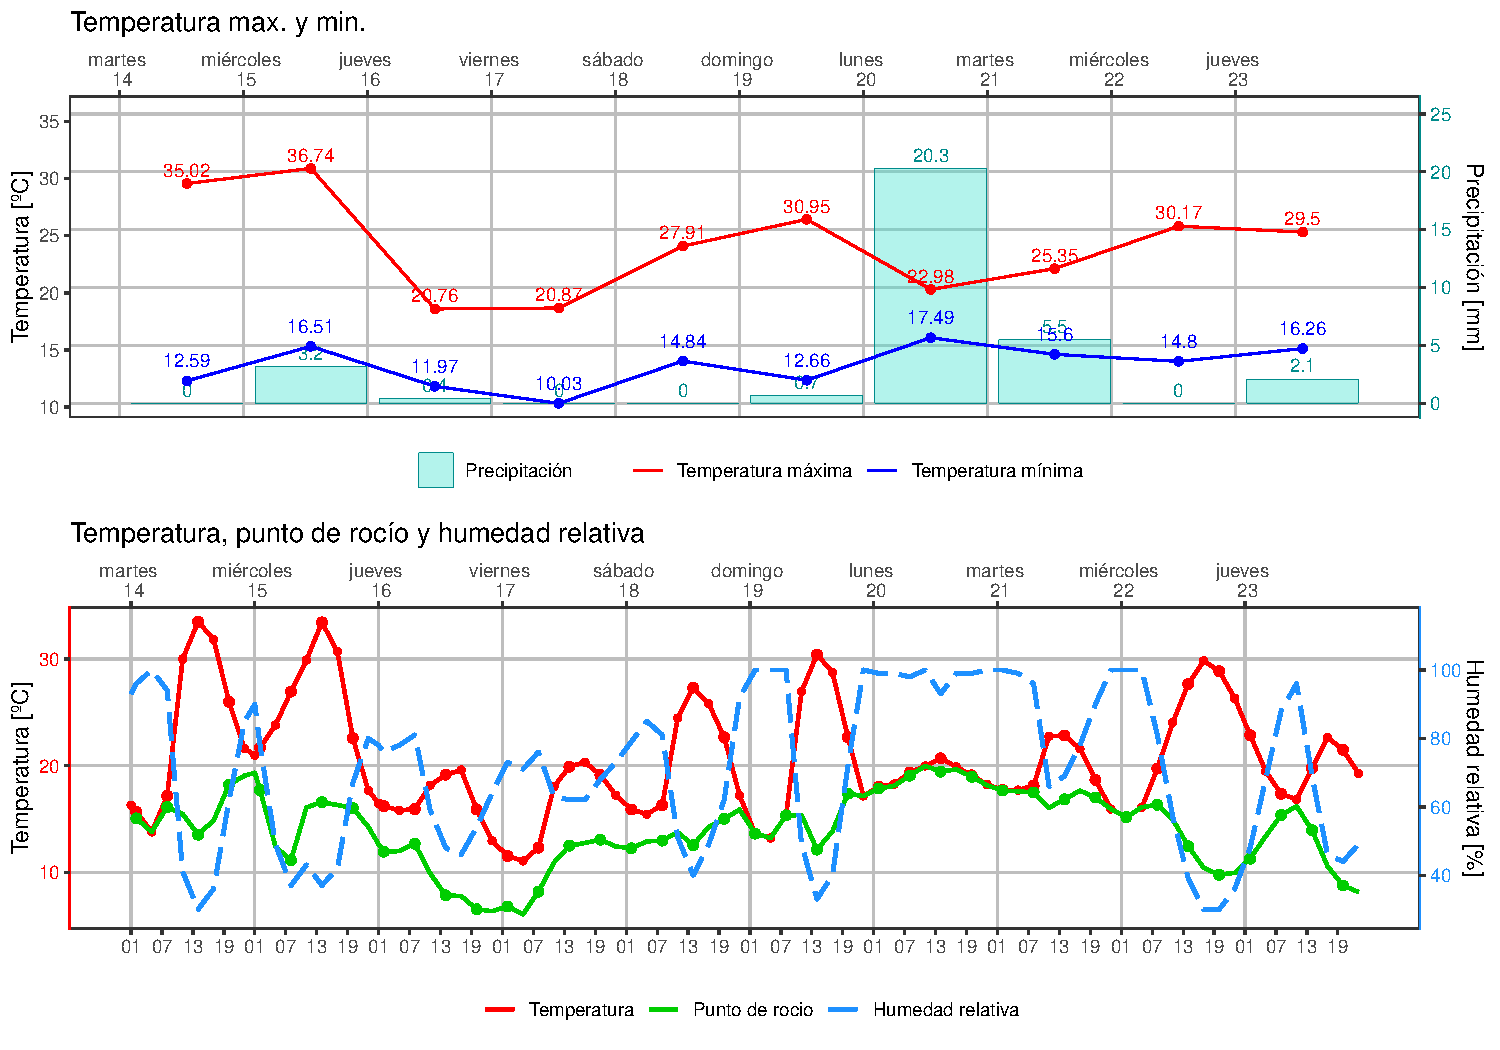
\includegraphics[width=\maxwidth]{figure/Figtemperatura-1} 

\end{knitrout}
\end{figure}

\begin{figure}
\begin{knitrout}
\definecolor{shadecolor}{rgb}{0.969, 0.969, 0.969}\color{fgcolor}
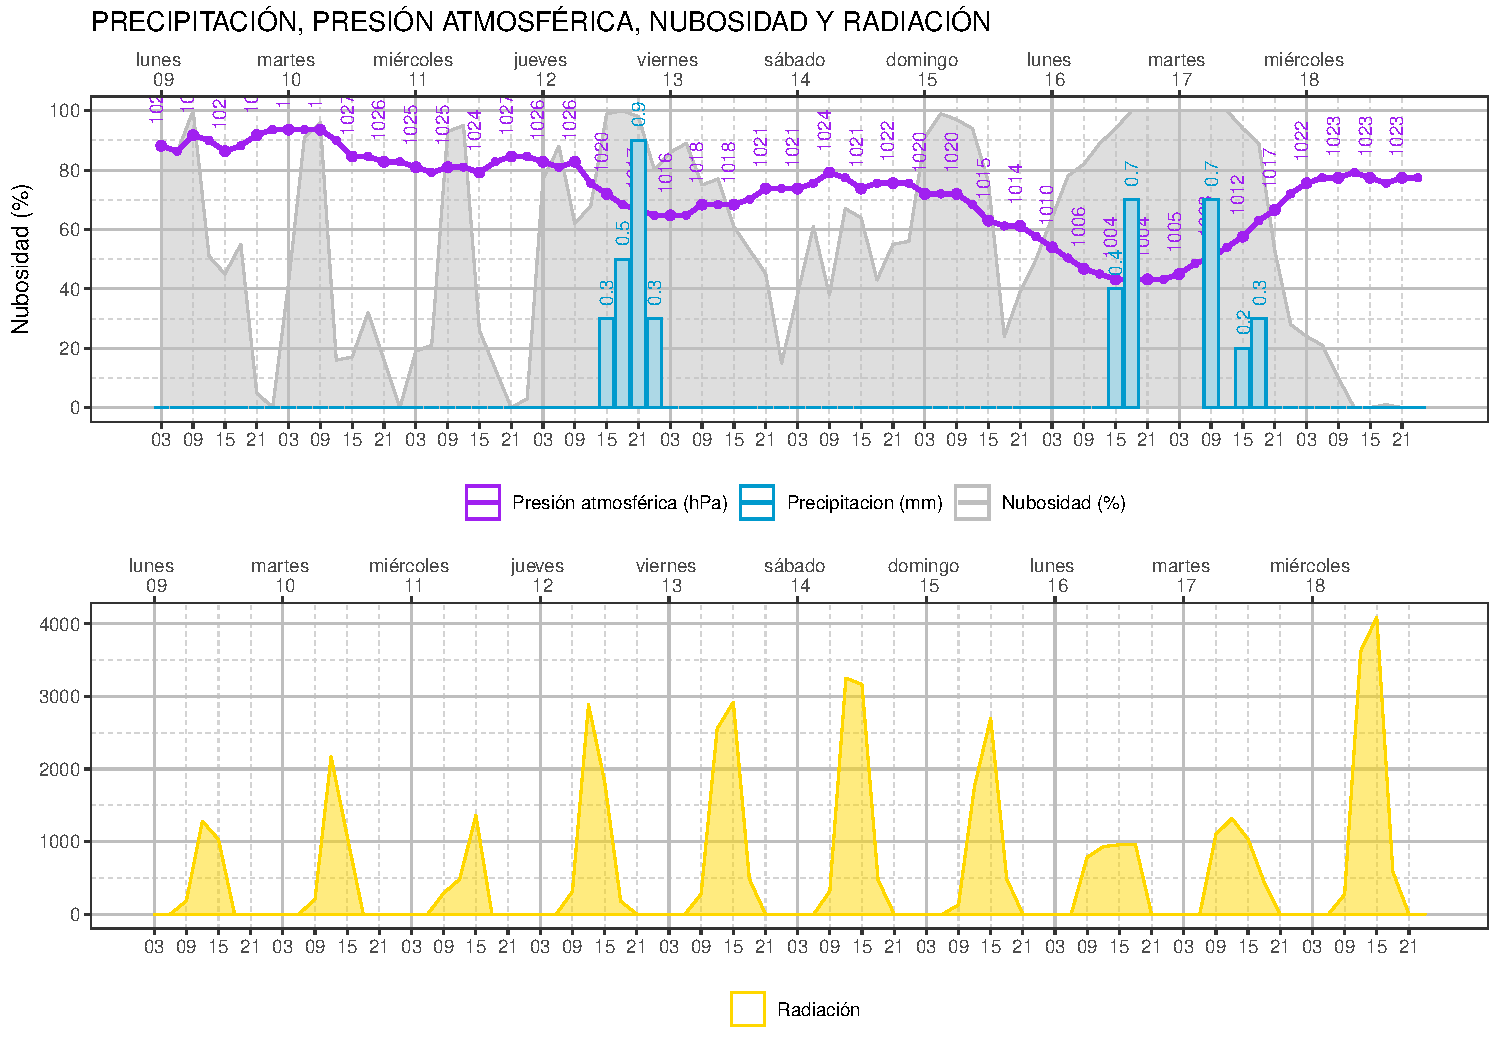
\includegraphics[width=\maxwidth]{figure/Figprecipitacion-1} 

\end{knitrout}
\end{figure}


\begin{figure}
\begin{knitrout}
\definecolor{shadecolor}{rgb}{0.969, 0.969, 0.969}\color{fgcolor}
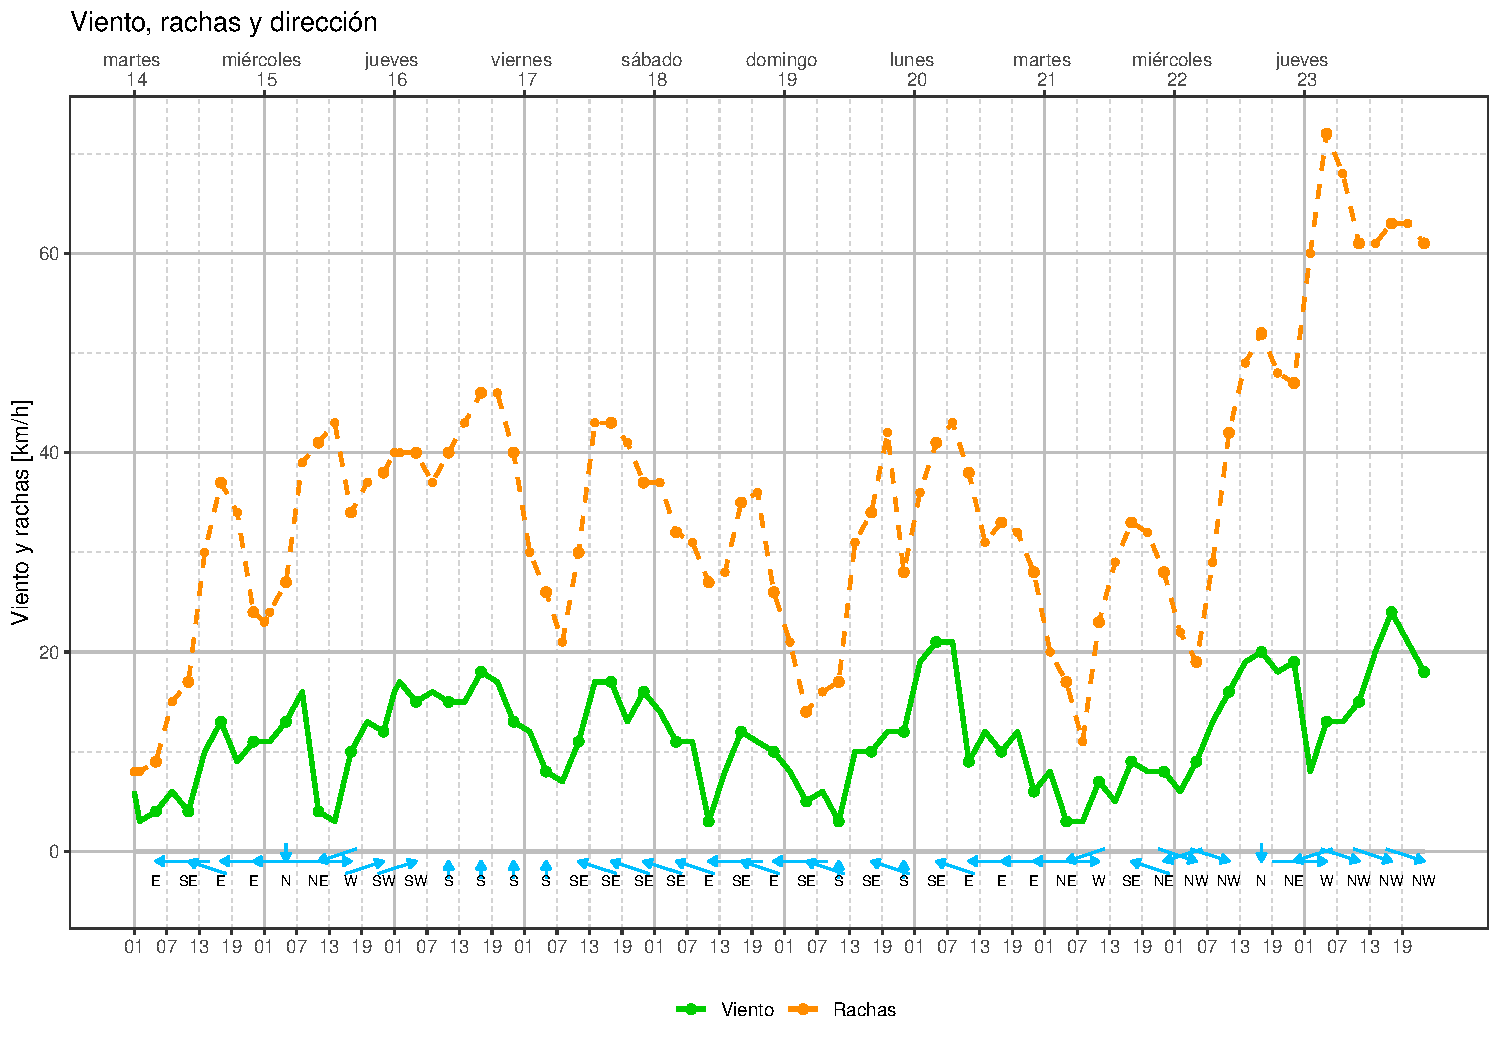
\includegraphics[width=\maxwidth]{figure/Figdir2-1} 

\end{knitrout}
\end{figure}


\begin{figure}
\begin{knitrout}
\definecolor{shadecolor}{rgb}{0.969, 0.969, 0.969}\color{fgcolor}
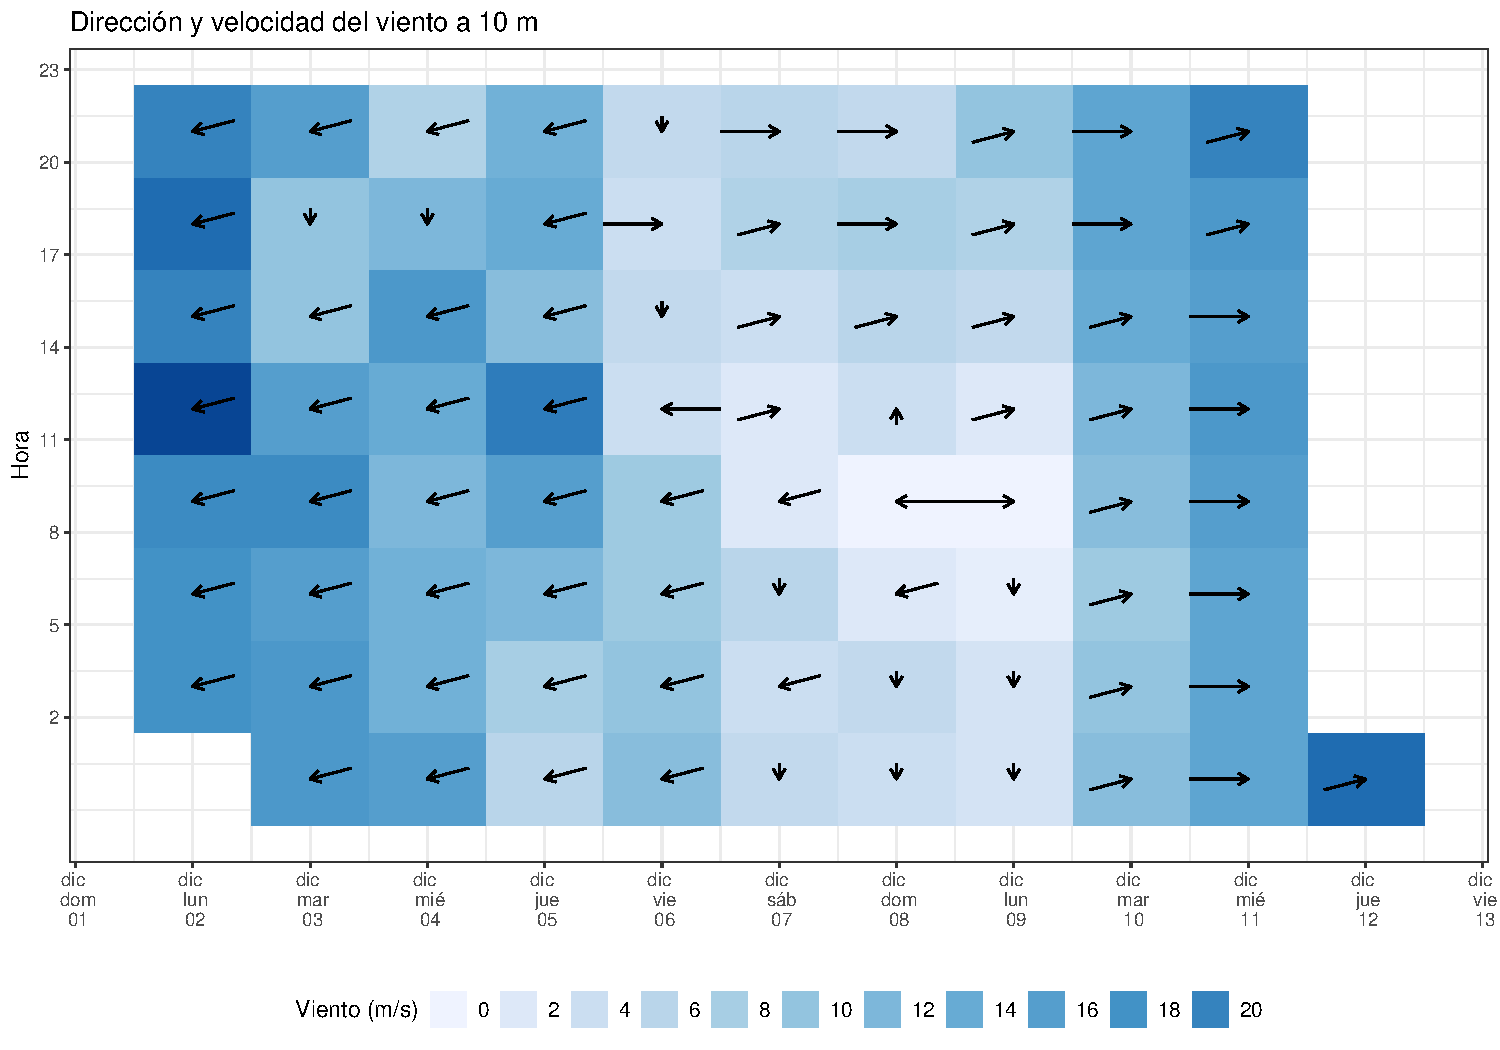
\includegraphics[width=\maxwidth]{figure/Figdir3-1} 

\end{knitrout}
\end{figure}




%<<CreateTable1, warnings=FALSE ,echo=FALSE, results = 'asis'>>=
%kktabla=cbind(kk$dateok,kk$presion,kk$nub,kk$hum,kk$precip)
%table_latex <- xtable(kktabla,caption = "cosas")
%print(table_latex,
%   latex.environments =  c("scriptsize", "center", "widestuff"),
%	          floating = FALSE
%		  )
%@


%\begin{figure}
%<<Figprec, echo=FALSE,fig.width=10>>=
%pnub <-ggplot(kk,aes(x=dateok)) +
%        geom_area(aes(y=nub),fill="grey",alpha=0.5) +
%        geom_line(aes(y=hum),col="#56B4E9",size=1.5)+
%        scale_x_datetime(breaks = date_breaks("1 days"))+
%        geom_text(aes(x=dateok,y=-8,label = nub), vjust = -1, size = 3, col="darkgrey", angle=90) +
%        geom_text(aes(x=dateok,y=-2,label = hum), vjust = -1, size = 3, col="#56B4E9", angle=90) +
%        labs(title="Nubosidad", subtitle="Humedad relativa (%)", x=" ", y=" ")+
%        theme(plot.title=element_text(size=12, color="darkgrey", lineheight=-1.5),
%                        axis.title.x = element_blank(), axis.text.x = element_blank(),
%                        plot.subtitle = element_text(size=12,color="#56B4E9"))

%ppresion <-ggplot(kk,aes(x=dateok)) +
%            ylim(min(kk$presion)-5,max(kk$presion)+5)+
%            geom_line(aes(y=presion),col="purple",size=1.2)+
%            geom_point(aes(y=presion),col="purple",size=1.5)+
%            geom_text(aes(x=dateok,y=presion, label=presion),col="purple",size=3, hjust=2)+
%            scale_x_datetime(breaks = date_breaks("1 days"))+
%            theme(plot.title=element_text(size=12, color="purple"))+
%            labs(title="Presión (hPa)", x=" ", y="")+
%            theme(axis.title.x = element_blank(), axis.text.x = element_blank())

%pprecip <-ggplot(kk,aes(x=dateok)) +
%        #geom_line(aes(y=precip),col="cyan3",size=1.5)+
%        geom_bar(aes(y=precip),stat="identity" ,col="cyan3",fill="cyan3")+
%        theme(plot.title=element_text(size=12, color="cyan3"))+
%        scale_x_datetime(breaks = date_breaks("1 days"),date_labels = "%b \n %a\n %d")+
%        geom_text(aes(x=dateok,y=-0.05,label = precip), vjust = -1, size = 3, col="cyan3", angle=90) +
%        geom_text(aes(x=dateok[40], y=0.15, label ="Pecipitación (mm)"),col= "cyan3",size=4)+
%        #geom_text(aes(x=dateok[4],y=-0.01,label = precip[4]), vjust = -1, size = 3, col="blue") +
%        #geom_text(aes(x=dateok[40],y=-0.01,label = precip[40]), vjust = -1, size = 3, col="blue") +
%        #labs(title="Precipitación (mm)", x=" ", y="",caption="Source: ECMWF")
%        labs( x=" ", y="",caption="Source: ECMWF")

%grid.newpage()
%grid.draw(rbind(ggplotGrob(pnub), ggplotGrob(ppresion),ggplotGrob(pprecip) , size = "last"))
%@
%\end{figure}


%\begin{figure}
%<<Figdir, echo=FALSE>>=
%tstep=seq(1,16)
%par(mfrow=c(4,4))
%for (i in tstep) {
%    plot(c(0,kk6h$u[i]),c(0,kk6h$v[i]),xlim=c(-1,1),ylim=c(-1,1),type="l", ylab="", xlab="",xaxt= "n", yaxt="n", main=paste(kk6h$dir[i]," H=", kk6h$date[i] ,sep=""),col="red")
%    axis(2, at=c(-1,0,1),labels=c("SW","W","NW"), col.axis="red", las=2)
%    axis(4, at=c(-1,0,1),labels=c("SE","E","NE"), col.axis="red", las=2)
%    axis(1, at=c(0),labels=c("S"), col.axis="red", las=2)
%    axis(3, at=c(0),labels=c("N"), col.axis="red", las=2)
%}
%@
%\end{figure}

\vspace{5cm}
\newpage

%<<CreateTable,  warnings=FALSE, echo=FALSE, results = 'asis'>>=
%kk=cbind(fecha[t3h], presion[t3h],temperatura[t3h], dir[t3h])
%table_latex <- xtable(kk6h,caption = "cosas")
%print(table_latex,
%   latex.environments =  c("scriptsize", "center", "widestuff"),
%	          floating = FALSE
%		  )
%@

\textcolor{meteoblue}{Informaci\'on}
Descripción de las variables meteorol\'ogicas
\begin{itemize}
\item Presi\'on atmosf\'erica
\item Precipitaci\'on. NOTA: PRECIPITACION HORARIA PRIMERAS 24H!
\item Nubosidad
\item Temperatura máxima y mínima
\item Punto de rocío
\item Direcci\'on del viento
\item Velocidad del Viento
\item \textbf{Radiaci\'on Solar}: Cantidad de energía acumulada en un periodo de tiempo y se mide en Julios/m$^2$
\end{itemize}
NOTA: La magnitud de cada variable se proporciona cada tres horas.
IFS (Integrated Forecasting System)

\end{document}
